%%% Ch.3: Methodology %%%
\chapter{Methodology and Implementation} \label{ch:method}
The problem of measuring the trustworthiness of communicating entities is an
essential aspect of any online system. This chapter states the problem of the
current system and follows on a discussion of a proposed endorsement system
where physically or digitally acquainted entities can endorse each other or
their presented information. The user types and their roles in the endorsement
system along with the design considerations are discussed. A system of smart
contracts is set up to specify the rules of interaction and method to aggregate
and compute the final global score for individual entities. Deployment of the
contract to the blockchain network and analysis of data storage both on and
off-chain is discussed. 

\section{Problem Statement}
To be able to rely on the trustworthiness of an entity as presented by any
online systems, the underlying reputation system needs to be robust and as
transparent as possible. The assurance that available information has not been
tampered with and correctness of claimed identity should be provided to sustain
minimal risk of fraud. The centralized nature of current online systems leaves
the propagation of reputation information vulnerable to external attacks as
well as internal modifications. As such, it fails to provide the guarantee of
reliable and immutable data. Additionally, the reputation systems do not take
into account the anonymity of participants, which is an essential attribute for
avoiding retaliation (e.g., a buyer may fear retaliation from a seller that
provided bad service) from providing honest negative feedback. This master's
thesis project proposes the use of blockchain technology for storage and
governance of reputation data to ensure reliable and publicly verifiable
information. By modeling trust among entities in a pseudonymous manner, the
proposed system also considers the users' anonymity requirement. 

\section{User stories \& System Requirements} \label{ch:UserStories}
This master's thesis project proposes a decentralized endorsement system to
model trust among participating entities. As the name suggests, the proposed
system allows participants to endorse each other to reflect their subjective
opinion about other participants. Thus, the two distinct roles of users in this
system are endorser (who sends an endorsement) and endorsee (who receives an
endorsement). The relation between an endorser and an endorsee is an
endorsement relationship. One might want to establish an endorsement relation
with other entities in the network based on physical or digital acquaintance.
\par
The acquaintance could be of the following form: 
\begin{itemize}
	\item Alice and Bob go to the same school/workplace, have worked on
		multiple projects together and therefore are confident of each other's
		reliability.
	\item Alice has dealt many times with Bob in an online shopping platform
		and always had a successful transaction outcome with him. In this
		interaction, Alice is sure that Bob is an honest seller and Bob is
		confident that Alice is a reliable buyer.
	\item Alice follows Bob on some social media and knows that Bob's article
		is good and sees lots of pre-research in his writing and is confident
		that Bob does not engage in spreading false news. 
\end{itemize}
%figure - System Context Diagram
\begin{figure}
	\centering
	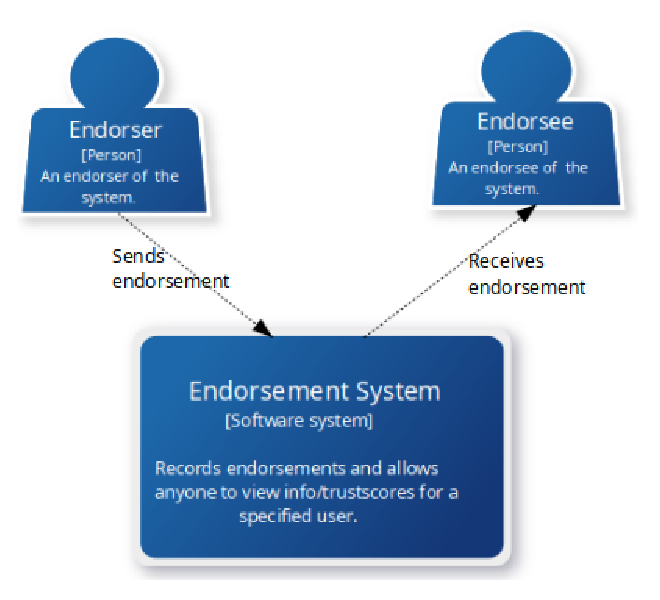
\includegraphics[width=0.7\textwidth]{Images/ContextLayer.eps}
	\caption{Context Layer}
	\label{fig:context}
\end{figure}
Based on Alice's previous experience with Bob, she is likely to endorse Bob on
the endorsement system. Thus, the endorsement relationship aims to depict the
direct, personal/interpersonal trust between entities. The endorsement system
seeks to offer a simple computation model to aggregate the endorsement
interactions and assign a reputation value to infer trustworthiness. If a
participant $A$ endorses a participant $B$, then it implies that $A$ trusts
$B$. As such, the domain of trust value in this system is binary. An entity $A$
is either endorsed or not endorsed by $B$ in the network. The
Figure~\ref{fig:context} shows the endorsement interaction between users
(endorser and endorsee) and the endorsement system.  In software development
paradigm, user stories~\cite{cohn2004user} provide an informal description of
the feature that the system can have from an end user perspective. Sketching
user stories for the endorsement system can help to define the roles and the
associated specific features for a given user role.
Table~\ref{table:userstories} presents the user stories for different user
types of endorsement system and follows a role-feature-reason
template~\cite{agile1}. The traceability column is used to trace back to that
specific feature when checking the fulfillment of requirements in
Section~\ref{fulfillment}. 

\begin{center} \label{table:userstories} 
	\begin{table}
	\begin{tabular} {| l | p{8cm} | l |}
		\hline
		\textbf{As an}  & \textbf{I need to be able to..}   & \textbf{Traceability} \\
		\hline
		\multirow{2}{*}{Endorser} & send an endorsement so that the endorsement
		is received by the endorsee.& R1
		\\\cline{2-3} 
		& remove endorsement so that the endorsement is removed from the
		endorsee.  & R2 \\\cline{2-3}
		& view a list of endorsees so that i can see from whom i have received 
		endorsements.& R3 \\\cline{2-3}
		& view/edit my personal information so that i can keep it up to
		date& R5 \\\cline{2-3}
		\hline
		\multirow{2}{*}{Endorsee} & view a list of endorsers so that I can see
		from whom I have received endorsements.& R3 \\\cline{2-3}
		\hline
		\multirow{2}{*}{other users} & compute the total endorsement
		impact (i.e., final computed score) of any registered members so that I
		can make an informed decision about the future transactions.
		& R4.1 \\\cline{2-3}
		& make a request to join the endorsement network so that I can start
		sending and receiving endorsements.  
		& R4.2 \\\cline{2-3}
		\hline
	\end{tabular}
	\caption{User Stories and Requirements}
\end{table}
\end{center}
\vspace{-15mm}
The users should be able to interact in the system based on their roles and the
features allowed by the role. The endorsement acts like a transaction message
that originates from a user account and is destined to another user account. As
such, the originator account is an endorser and the destination account is that
of endorsee. Every user maintains two separate lists of participants that they
have interacted with. The first is the list of endorsers, that consists of the
account addresses of all the participants that have endorsed the user. The
second is the list of endorsees, that consists of the account addresses of all
the participants that have been endorsed by the user. Account address acts like
an identifier to the user. Based on this definition, we can lay out the system
requirements. \par
%and the rationale for user interaction. \par
The functional requirements can be listed as: 
\begin{enumerate}
	\item It must be impossible to make an endorsement if the endorser and
		endorsee belong to the same account. \newline
		This requirement enforces a restriction that entities cannot endorse
		themselves.  
	\item It must be impossible to remove endorsement from a participant if the
		transaction initiator (account calling remove endorsement) is not in
		the list of endorsers for the participant.
	\item All the endorsements must be stored such that, it is possible to see: 
		\begin{itemize}
			\item account address of endorser and endorsee for the given
				endorsement. 
			\item degree of incoming and outgoing connections for all endorsers
				and endorsees.
		\end{itemize}
	\item There must be a way to link the account address (which is the public
		key address of an account) to their corresponding global score (the
		final score used to infer the trustworthiness).
	\item It must be possible for a participant to edit their personal
		information such as their username. Since the endorsement system does
		not rely on the real-world identity of the participants, they should be
		allowed to edit or update their personal information at will. The trust
		score is linked to a unique identifier and cannot be actively updated
		by any participant.  Computation of trust scores is explained by
		Section~\ref{sec:endorsementModel} which discusses the design of the
		endorsement system in detail. 
\end{enumerate}
The non-functional system requirements relate to the system's architecture and
can be listed as:
\begin{enumerate}
	\item Security: Solidity has a list of known bugs~\cite{soliditySecurity}
		and recommendations on security considerations~\cite{solidityBugs} for
		writing smart contract code. The smart contract code for endorsement
		system should take into account minimal security considerations to
		avoid the relevant possible bugs. 
	\item Reliability: The  trust and reputation information should be stored
		in an immutable and publicly verifiable manner.
	\item Trust metrics should correctly describe the actual trust score of the
		nodes. The definition of honest or malicious interaction based on the
		endorsement model should be reflected by the final score assigned to
		the participant. As such, the nodes showing honest behavior should have
		a better score than the malicious ones.   
\end{enumerate}

\section{The Model - Endorsement Network}\label{sec:endorsementModel}
%\begin{figure}
%	\begin{center}
%		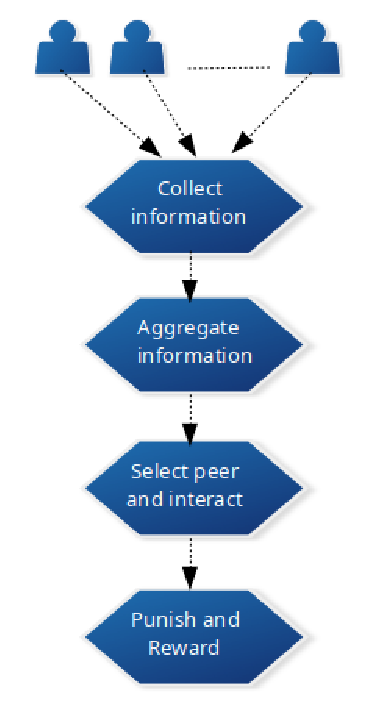
\includegraphics[width=0.4\textwidth]{Images/TrustReputationSteps.eps}
%		\caption{Trust and Reputation Model steps taken from~\cite{marmol2009security}}
%		\label{fig:truststep}
%	\end{center}
%\end{figure}
The figure~\ref{fig:truststep} shows the steps required to have a complete
"trust and reputation system" and is based on ~\cite{marmol2009security}. Among
these steps, the endorsement system only concentrates on the first two steps,
collection, and aggregation of information. The information in the endorsement
system refers to the endorsement interactions between entities and values they
represent. The last two steps of selecting a peer and getting punished or
rewarded are based on a transactional system. As implementing the
transaction-based system is not the main task of this project, feedback based
on the success or failure of a transaction is purely based on an assumption
about the transaction network. \par 
%\begin{wrapfigure}{l}{0.6\textwidth}
\begin{figure}
	\begin{center}
		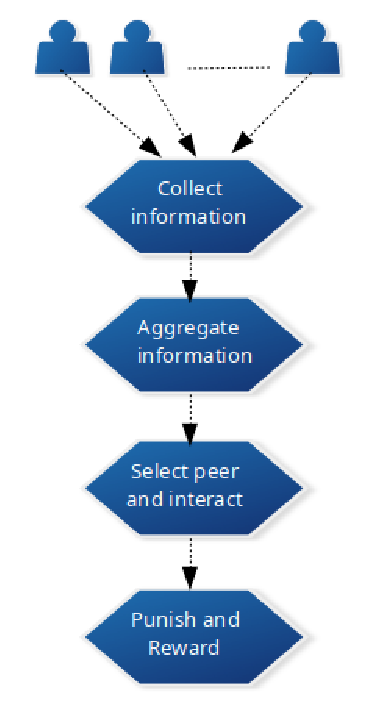
\includegraphics[width=0.3\textwidth]{Images/TrustReputationSteps.eps}
		\caption{Trust and Reputation Model steps based
		on~\cite{marmol2009security}.}
		\label{fig:truststep}
	\end{center}
\end{figure}
%\end{wrapfigure}
\subsection{Design of Endorsement System}
The design of the endorsement system is based on the requirements mentioned in
Section~\ref{ch:UserStories}. This section explains the design considerations
that were taken into account for the endorsement system. The
Figure~\ref{fig:components} shows different components of the endorsement
system and how the users interact with them. Each of the components is
described in Section~\ref{sec:implementation}. The endorsement system allows
participants to endorse each other based on their trust opinion. Before
discussing the endorsement relationship, it is essential to understand the
characteristics of trust that is taken into account by the system. Abdul-Rahman
A, Hailes S.~\cite{abdul1998distributed} have discussed these properties of
trust in their study of a distributed trust model. \par
%First, let us make the following definitions that will be used later:
%\begin{itemize}
%	\item A $\overset{endorses}{\implies}$ B, represents the relationship, $A$
%		endorses $B$.
%	\item A $\overset{trusts}{\implies}$ B, represents the relationship, $A$
%		trusts $B$, i.e., $A$ believes that $B$ is trustworthy.
%\end{itemize}
%The endorsement system considers the following characteristics of trust: 
%\paragraph{Trust is Dynamic:} This characteristic relates to the requirement of
%allowing a user to remove endorsement previously given.
%\begin{equation}
%	(A \overset{endorses}{\implies} B) \implies (A \overset{trusts}{\implies} B)
%\end{equation}
%endorses$(A, B)$ shows the trust relationship at a given time $'t'$. If $A$
%decides that $B$ is not trustworthy for any reason then $A$ should be allowed
%to do that. In which case, the endorsement information for both $A$ and $B$
%must be updated to reflect the current state. 
%\paragraph{Trust is asymmetric:} 
The endorsement system considers the following characteristics of trust:
\paragraph{Trust is Dynamic:}The trust between two individuals can change over
time. Thus, if an entity $A$ endorsed $B$ at a time $t_{1}$, then $A$ can take
back that endorsement from $B$  at any time $t_{2}$ such that $t_{2} > t_{1}$.
The endorsement system then updates this information for both $A$ and $B$ to
reflect the current state.  
\paragraph{Trust is asymmetric:}Trust relationship does not necessarily have
to be bi-directional, i.e., $A$ trusts $B$ does not always imply that $B$
trusts $A$ too. Therefore, the endorsement system does not enforce any
restriction on the endorsement relation between two entities to be asymmetric.
This attribute is demonstrated in the endorsement system by not requiring a
participant to endorse back the endorser, i.e., if $A$ is endorsed by $B$, then
it is entirely up to $B$ to either endorse back $A$ or not.
\paragraph{Trust is not transitive:}The endorsement system does not consider
the transitive trust path that can exist between endorser and endorsee. The
only way an endorsement relation can be made between two entities is via direct
endorsement. There exist trust metrics that are modeled based on the
transitive nature of trust. Depending on the context where the trust metrics is
applied, this attribute can be meaningful, e.g., in
eigentrust~\cite{kamvar2003eigentrust}, a peer $i$ is assumed to have a higher
belief in the opinion of a peer from whom he/she has received authentic
(non-malicious) files. Depending on the behavior of participants in the
network, the transitive trust can have a positive or negative outcome. If the
majority of participating nodes happen to be malicious actors (or collection of
nodes that believes in false information) then the trust transitivity could
result in the spread of incorrect information faster.  Thus, to avoid the risk
of spreading false beliefs, the endorsement system does not consider the
transitive trust for the computation of a trust score.  Christianson B,
Harbison WS~\cite{christianson1996isn} have studied the non-transitive nature
of trust in their study. 
%Thus, most of the sections is based on the smart contract logic for the
%endorsement model and discussion on the possibility to be used by other
%transactional systems.  
%
%The initial assumption on endorsement system is that all nodes are honest and
%as such receive equal points that they can spend at will, once registered on
%the network. These received points are the consumable power that keeps
%depleting with every endorsement connections made along the way. As can be seen
%in figure~\ref{consumablePoint}, these points follow a convergent sequence that
%converges to the limit zero as the number of connection `n' increases. As such,
%increasing the number of connections alone will not be enough to achieve a
%higher impact on the network.
\subsection{Computation of Total Endorsement Impact (TEI)} 
The endorsement system records all the endorsement interactions between
endorsers and endorsees. This information is aggregated for individual entities
in the system to assign a global trust score. We call this score a total
endorsement impact as it is supposed to represent the total impact a node has
made on the endorsement network. First, we define the terminologies related to
the endorsement system and present the method to compute the value for total
endorsement impact.\newline 
\textbf{{\acrshort{nEG$_A$:}}} \ac{nEG} by a participant $A$. \newline
\textbf{{\acrshort{nER$_A$:}}} \ac{nER} by a participant $A$. \newline
\textbf{ratio$_A$:} represents the ratio of \acrshort{nEG$_A$} to
\acrshort{nEG$_A$}. This value can be used to ensure that the sent and received
endorsement are not far off from each other. ratio$_{A}$ is always less than or
equal to 1 and is given by:   
\begin{equation}
	ratio_A = \frac{min(nEG_A, nER_A)}{max(nEG_A, nER_A)}
\end{equation}
\textbf{\acrshort{CP}$_A$:} represents the \ac{CP} of a participant $A$. Every
node that joins the network receives an equal amount of consumable points from
the endorsement network. This value keeps depleting with each outgoing
endorsement connection. 1 being the initial consumable points received by
participant $A$, $CP_{A}$ is given by $\frac{1}{nEG_A}$.\newline
\textbf{\acrshort{TRP$_A$}:} This corresponds to \ac{TRP}, which is the
accumulated sum of consumable points received by $A$ from his/her endorsers.
\newline
If $E = \{e_{1}, e_{2}, e_{3}, ......., e_{n}\}$ is a set of endorsers for a
peer $A$ and the size of $E$ is $n$, then the $TRP_{A}$ is given by:
\begin{equation}
	TRP_A = \sum_{i=1}^{n}CP_{e_{i}}
\end{equation}
Finally, the \ac{TEI} made by $A$ is given by: 
\begin{equation}
	TEI_A = ratio_A \cdot TRP_A
\end{equation}

\begin{figure}
	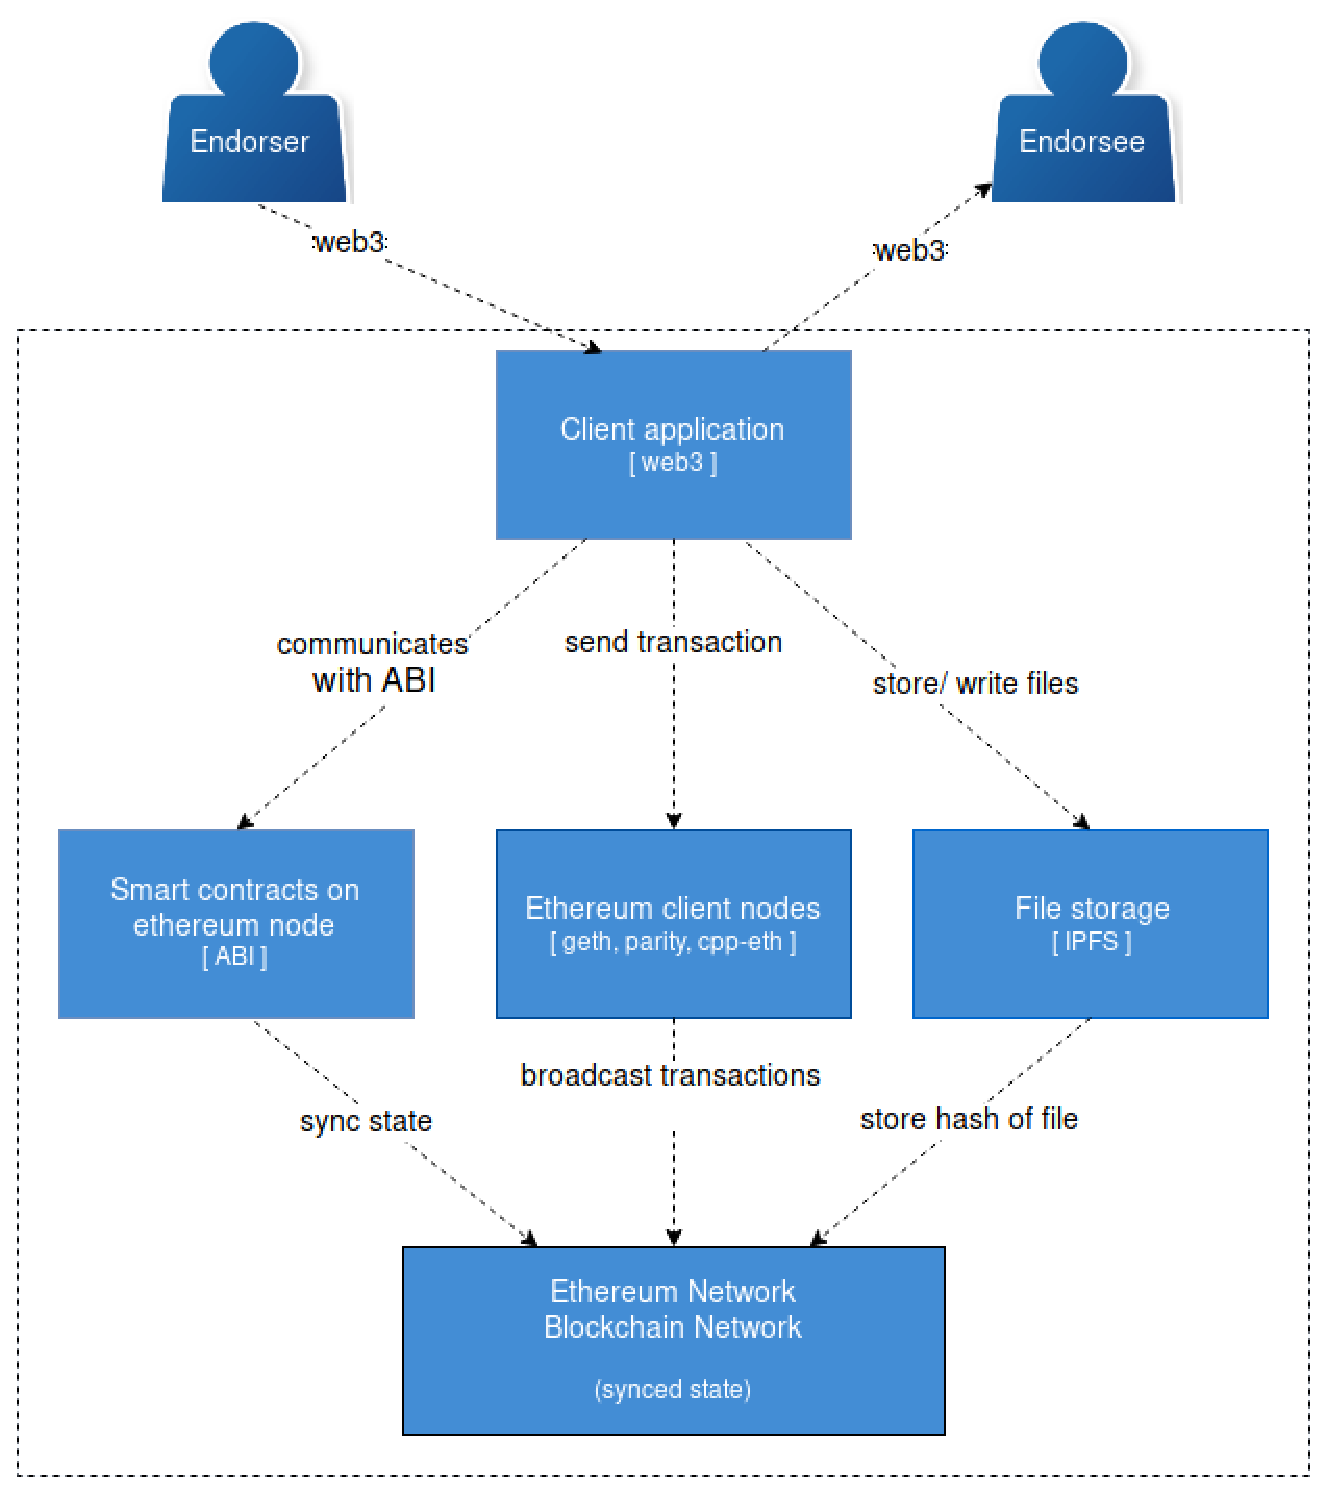
\includegraphics[width=0.9\textwidth]{Images/components.eps}
	\caption{Components of Endorsement System}
	\label{fig:components}
\end{figure}
\subsection{Design Considerations}
The design of the endorsement system considers several possible behaviors that
can result from the interaction between nodes, both honest and malicious. Any
node that tries to manipulate (to inflate or damage the reputation) the trust
score assigned by the endorsement system is a malicious node. For instance, a
node can create multiple accounts to send multiple endorsements to a specific
account. To limit dishonest behaviors while encouraging honest interactions,
some assumptions and definitions were made from a game theoretic perspective of
a behavioral outcome. Game theory~\cite{myerson2013game} is a study of
mathematical models of conflict and cooperation between intelligent rational
decision-makers. The game refers to any social situation that involves two or
more individuals, and players refer to the individuals involved in the game.
Game theory makes assumptions that each player's objective is to maximize the
expected value of his payoff, which is measured in some utility scale.
Transferring this notion to the endorsement system, the players being the
participants of the endorsement network. The assumption is made that the
objective of each participant is to maximize the trust score in the endorsement
system. Based on this assumption, some definitions were made to derive the
network influencing factors. As such, these factors can encourage honest
behavior while limiting malicious interactions in the endorsement system. 
The network influencing factors based on these assumptions are:
\paragraph{False endorsement with pseudonymous identities:} Availability and
public verifiability of reputation information is one of the primary concerns
of endorsement system. As such, the system needs a public permissionless
blockchain network which allows anyone to join the network and start sending
endorsements immediately to whoever they wish to. This creates the possibility
for an entity to create multiple pseudonymous identities with an aim to inflate
their impact on the network by increasing the number of endorsements (given or
received). There is no straightforward way to detect and stop such behavior.
However, if doing so does not provide any significant advantage, then the
assumption is that a rational decision would be not to do it. The endorsement
network allocates an equal amount of consumable points to each user that joins
the endorsement network. This value keeps depleting with each outgoing
endorsement connection made along the way. As can be seen in
Figure~\ref{consumablePoint}, the consumable points follow a convergent
sequence that converges to the limit 0 as the number of connection '$n$'
increases. While there is no limit to the number of endorsements a participant
can give, as this number increases, the value of consumable point decreases.
This value accumulatively results to the total received points for the
respective endorsee. Consider a scenario where a participant $A$ receives
endorsements from 3 endorsers, each having 2 outgoing connections. In this
case, the value of $TRP_{A}$ is 1.5. If the endorsers of $A$ instead had 5
outgoing connections each, then the $TRP_{A}$ would be only 0.6. \ac{TRP} is
one among other factors that contribute to making a better impact score on the
endorsement network. As a rational endorser, one would be willing to make fewer
meaningful endorsement connections that can contribute a larger value than to
make many connections with minimal value. As such, the convergent behavior of
consumable points is assumed to stop a participant from making too many
endorsements. 
\begin{figure}
	\centering
	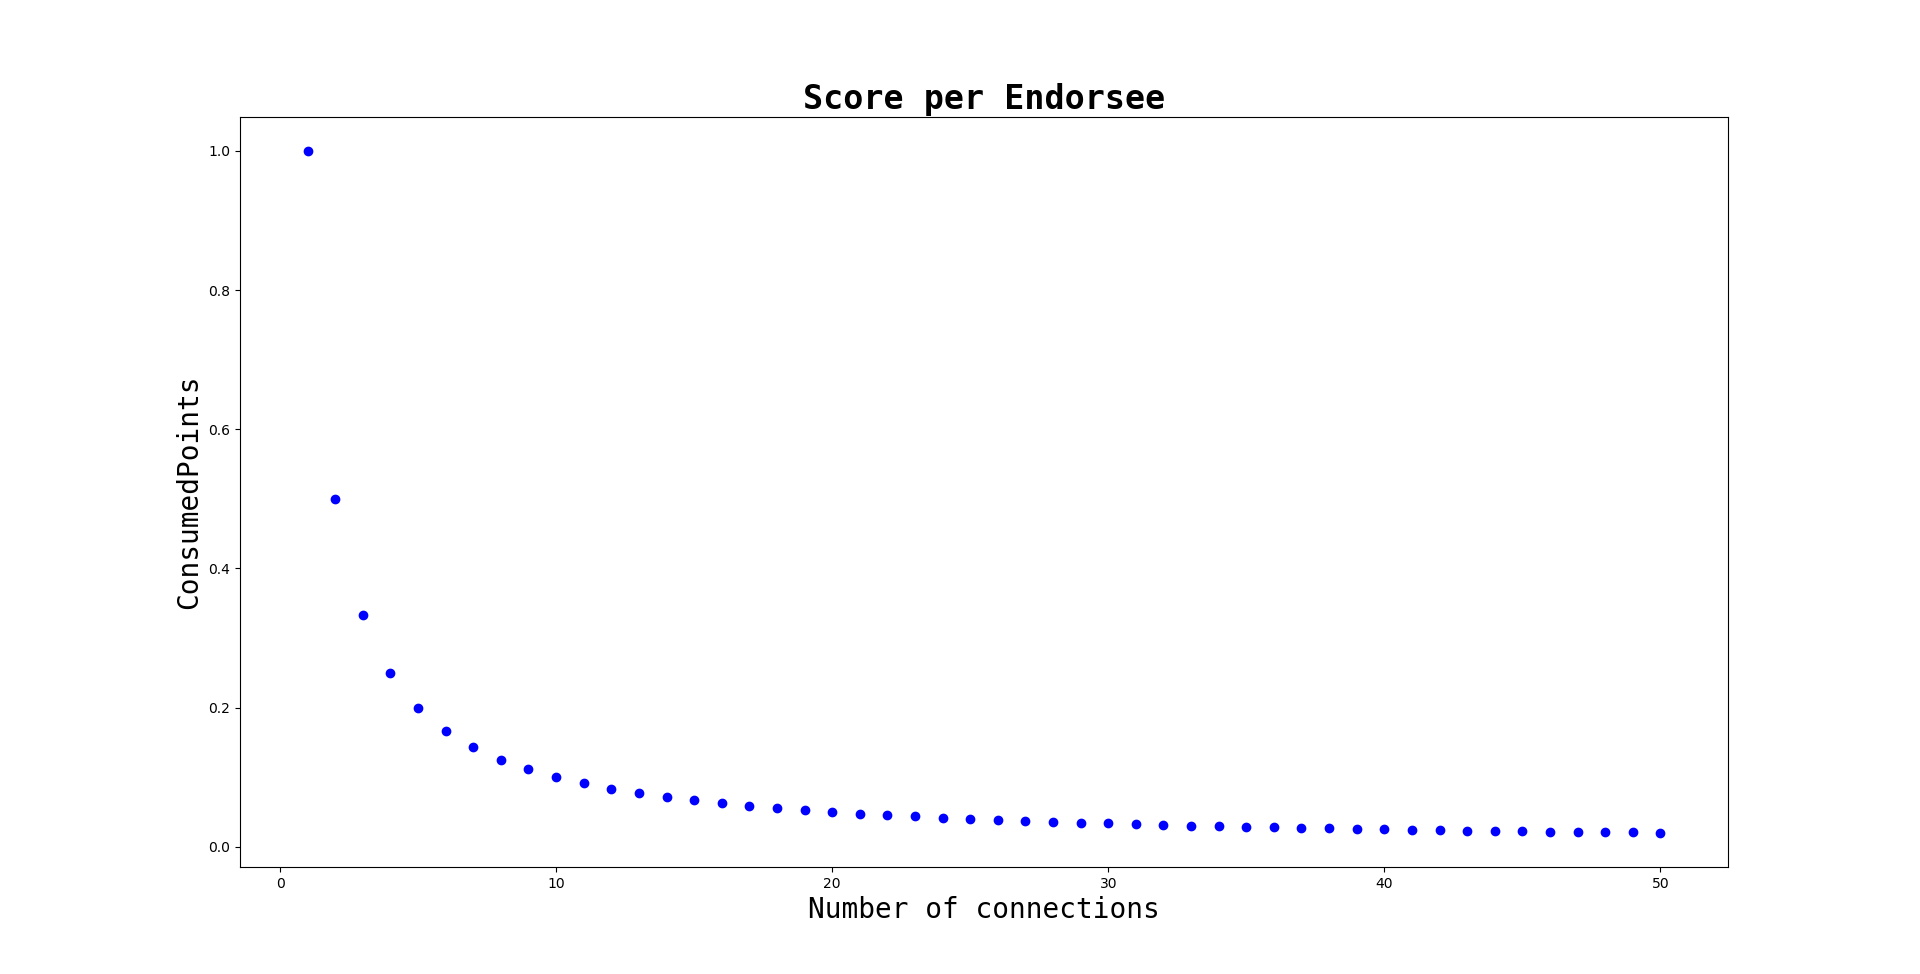
\includegraphics[width=1.0\textwidth]{Images/consumedpoints.eps}
	\caption{Convergent behaviour of consumable points as '$n$' increases.}
	\label{consumablePoint}
\end{figure}
\paragraph{Transaction Cost:}The endorsement system makes use of Ethereum as a
blockchain infrastructure. As mentioned earlier, every operation executed on
ethereum consumes a certain amount of gas, which is a scarce resource. The account that makes a call to endorse function is responsible for paying all the
required gas costs. The endorse transaction if executed successfully updates
the state variables \ac{nEG} and \ac{nER} for the source and destination
account addresses. While the gas cost may not seem too high for making one
transaction, a malicious node with multiple pseudonymous accounts needs to pay
the gas cost of all transactions initiated from all the pseudonymous accounts.
For instance, given the interaction graph in Figure~\ref{fig:subgraphexample}, if
Alice is an honest node, then she only needs to pay for the operation of two 
transaction. On the other hand, if both Bob and Charlie are the pseudonymous
identities of Alice, she needs to pay for six transactions. As the number of
pseudonymous accounts increases, the cost for maintaining the trust score on
each (or one target) account also increases. Therefore, it is possible
that the pseudonymous accounts exchange ether with each other for having the
balance required to pay the transactions cost. This information can be publicly
verified by anyone on the blockchain network to view the chain of ownership. If
some interactions in the endorsement network look unusual (e.g., if an account
has received too many calls for removing endorsements), then one could look up
details as such. This kind of information acts as an additional factor that
might be useful to look up before making a transaction decision. 
\begin{figure}
	\centering
	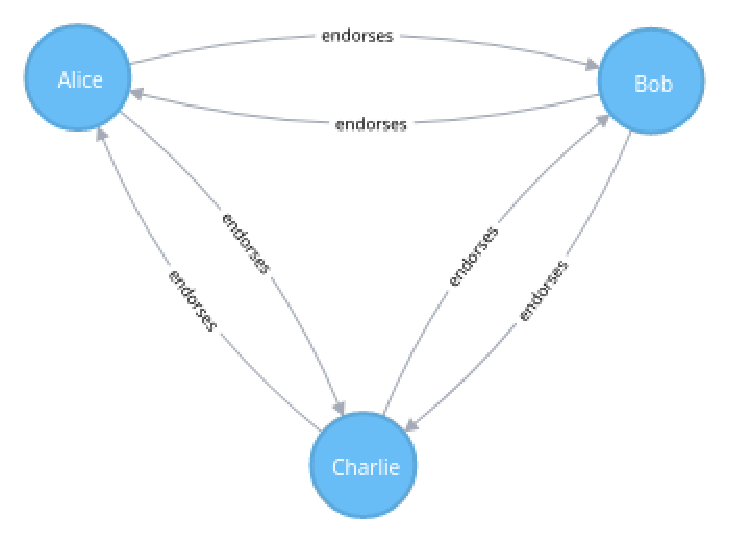
\includegraphics[width=0.6\textwidth ]{Images/subgraphexample.eps}
	\caption{Interaction between participants that endorses each other}
	\label{fig:subgraphexample}
\end{figure}
A successfully executed endorsement transaction modifies the \ac{nEG} and
\ac{CP} for the source account and \ac{nER} for destination account. Besides
the source and destination account, the state of \ac{TRP} for all past
endorsers of source account also needs to be modified. Therefore, a node needs
to keep track of all its neighboring (endorsers) nodes as well for correctly
computing the \ac{TEI} value. To get the total sum of \ac{CP}, it requires
iterating through the list of endorsers' accounts. The larger the size of this
list, the larger would be the cost of the computation. While it is possible to
iterate through the list of items in an array, Solidity does not generally
recommend doing so. The reason being that an unbounded loop can grow too large
and exceed the block gas limit, thereby causing the contract to be stalled.
Regardless of the amount of gas spent, the function call will not succeed. We
could assume that the list may not grow too big because a rational agent would
try to limit their endorsement connections to contribute a larger value to
other nodes in the network. Another reason we can assume so is that there is a
limit to the number of entities that one can make trust decisions about.
Dunbar's number~\cite{hill2003social}~\footnote{Dunbar's number is a suggested
	cognitive limit to the number of people with whom one can maintain stable
	social relationships—relationships in which an individual knows who each
	person is and how each person relates to every other person.} says that
	there is a limit of 150-200 stable social relationships that humans can
	maintain. A study by Dunbar, R. I. (2016)~\cite{dunbar2016online} suggests
	that the growth of online media and interactions still do not overcome
	those limitations. \par 
If we want to avoid relying on assumptions and expect the list to grow larger,
there are a few ways to approach this issue. One way to address this is by
setting an upper bound to the number of connections that a node can have.
Another way to approach this problem without setting a threshold value is to
move the computation to a non-blockchain platform. All the variables necessary
to compute the \ac{TRP} and \ac{TEI} can be stored and updated on blockchain as
a publicly verifiable information. The computation can be done on the
client-side using language such as javascript and the client can compute the
final score.  
\paragraph{Free riders problem:} The endorsement system is supposed to be a
voluntary contribution network where entities can endorse each other.
Therefore, the goal is to maintain a balanced ratio of incoming and outgoing
endorsement connections. This is enforced in a way that if a node does not
maintain the ratio then the \ac{TEI} does not increase to make a significant
impact on the network. This factor also discourages Sybil nodes because each
identity needs to have an almost equal bi-directional connection. If one is
only receiving from their pseudo identity that does not have too many
connections, then the impact is ignorant and thus not worth the effort.
\subsection{Rewards and Punishment}\label{rewardpunishment}
The computation of a global score on the endorsement system is based on the
subjective opinions of participants about each other. For the score to reflect
accuracy in computing the probability of success for a real-world transaction,
the score has to be updated based on some objective measure. As mentioned
earlier, the endorsement system only considers the two steps of trust and
reputation system. The complete steps can be seen in Figure~\ref{fig:truststep}
in Section~\ref{sec:endorsementModel}. The reward and punishment relate to the
fourth step which is based on a transactional outcome. Since the development
and analysis of transactional network is not part of this thesis project,
updating the trust score based on transactional feedback is not performed. A
transactional network can retrieve the information on the endorsement system to
provide additional conformity to its user about the reputation of an entity in
question. Say, Alice is registered on Endorsement network and has made a decent
score. If she wants to sell a product on a transaction network, she can claim
the trust score she has on the endorsement system. Anyone can verify the claim
by checking the score that corresponds to her public address. If both Alice and
buyer are registered on the endorsement network, they can send a signed message
to each other using their private key to prove the ownership of the address
with a good score on the endorsement network. In case the buyer is not
registered on the endorsement network, then Alice can prove the claim by
signing a cryptographic challenge with her private key. \par 
The notion of reward and punishment is an important one to reflect the current
trust status of a peer. There are several ways one can reward or punish a node
for its transactional behavior. For instance, a seller that failed to provide a
good service for a certain amount of time (e.g., received five negative
feedback continuously) could be punished. One simple method to punish the node
would be by reducing the trust score made so far by 50\%. Additionally, the
nodes that endorsed an untrustworthy node could also be punished by reducing
its trust score by 25\%. Reducing the score made so far by a certain percentage
will affect the users' reputation in the network. Anyone can see and verify
this information. Similarly, punishing the endorser can encourage a user to be
more careful about the trust decision they make.  

\section{Implementation} \label{sec:implementation}
There are several components that make up the endorsement system. The process
of sending the endorsement transaction from the client's browser to executing
the contract code that can change the blockchain state is discussed in this
section. It concludes with the discussion on storage of data and variables,
blockchain network and consensus mechanism.

\subsection{Smart contracts} \label{subsec:smartcontracts}
The process of starting up the node and deploying the contract to the
blockchain network is given by Figure~\ref{fig:startup}. To compile the
solidity code, solc~\cite{} compiler can be used. A successful compilation will
give a binary representation of compiled EVM bytecodes and an ABI (Application
Binary Interface). The binary output can be deployed to the blockchain network,
after which the contract will get an address and the bytecode is stored on
ethereum. ABI is a .json file that acts as a layer of translation for
interacting with the deployed smart contracts and calling the functions. We can
then start invoking contract's code using web3 API. For the compilation script
and list of smart contracts, the reader is directed to
Appendix~\ref{smartcontracts} and~\ref{ethapplication}. A single contract that
includes all the functionalities of the endorsement system is written as an
endorsement contract. Other contracts to set the owner of the contract and
allow the possibility to kill it is based on recommendations from
zeppelin-solidity~\cite{zeppelin-solidity} and its reusable code. \par
\begin{figure}
	\centering
	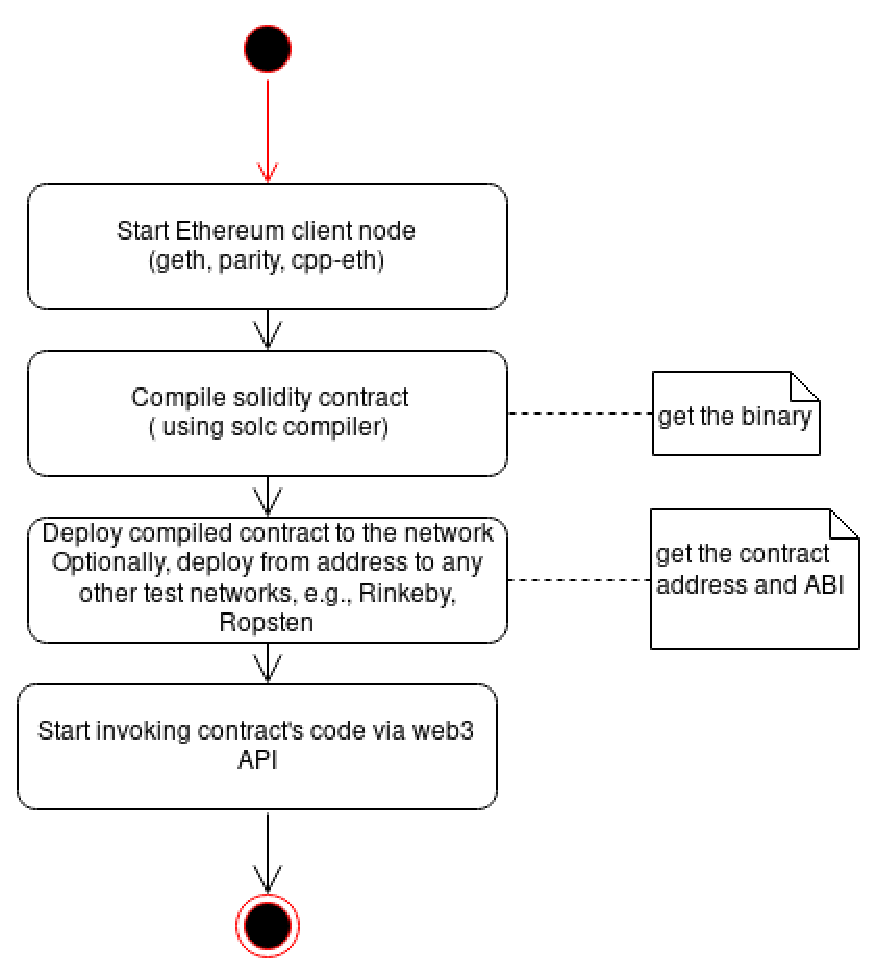
\includegraphics[width=0.6\textwidth]{Images/DeployContract.eps}
	\caption{Deploy solidity contract on the blockchain network}
	\label{fig:startup}
\end{figure}
The list of contracts written for the endorsement system and its
functionalities are: 
\paragraph{Ownable:} tracks the owner of the contract by setting the address of
owner.
address.
\paragraph{Killable:}inherits from Ownable and allows the owner of the contract
to destroy the contract.
\paragraph{Endorsement:}inherits from Ownable and killable. It specifies the
core logic of the endorsement system. The method to join endorsement network,
make endorsement interactions and request trust score of an entity are separate
functionalities of this contract. Each of these methods is discussed below. 
\paragraph{New participants:}sets participant and stores their information.
It maintains the records of all the participants and an index to access/query
their information. When a user invokes the code to join the endorsement
network, it stores the address of the user account that initiated the call and
sets it as the participant. An index to access each participant is maintained
that can be used to query the state. 
\paragraph{Endorsement:}allows participants to send endorsement transaction to
the network. When the endorsed method is invoked by a user account, the state
variables ~\ac{nEG} on the account that initiated the transaction gets
incremented. Similarly, the ~\ac{nER} for the account specified by the
transaction data. The list of endorsers and endorsees is updated for both the
accounts. 
\paragraph{ComputeImpact:} allows anyone to compute the total endorsement
impact given the address of a participant. When this method is invoked, the
\ac{TRP} for the given participant is calculated by accumulatively summing the
\ac{CP} of the list of endorsers.  
\subsection{Client Application} \label{clientapp}
\begin{figure}
	\centering
	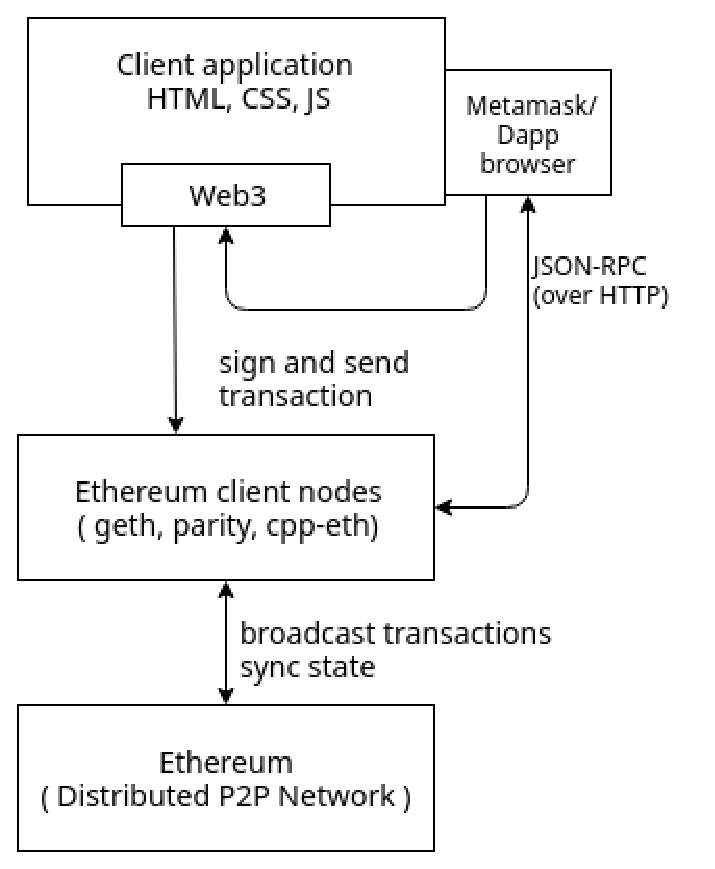
\includegraphics[width=0.5\textwidth]{Images/ClientApplication.eps}
	\caption{Client Application}
	\label{fig:ClientApp}
\end{figure}
The interaction between the client application and ethereum nodes is given by
Figure~\ref{fig:ClientApp} in Section~\ref{clientapp}.
Reactjs~\footnote{https://reactjs.org/} was used for front-end development of
endorsement application. The endorsement contract that performs the endorsement
logic was deployed to Ethereum test network,
Rinkeby~\footnote{https://www.rinkeby.io/#explorer} which can be accessed
publicly and the deployment steps can be seen in Appendix~\ref{ethapplication}.
The client application makes use of web3~\cite{web3}, which is a javascript API
that allows clients to interact with a local or remote ethereum node. A user
willing to interact with the endorsement system can submit the transaction via
a client application. The client application retrieves the required detail of
the user from the key store, and signs the message with users private key and
submit the transactions over to the client node. The client node executes the
contract code that corresponds with the transaction message. A successful
execution of the contract method would change the relevant states. One of the
miner nodes would pick this transaction, broadcast it over to the blockchain
network, and the transaction thus stays as an immutable and publicly verifiable
information in the blockchain. 
%\paragraph{Context Layer} \label{Contextlayer}
%The users (endorsers or endorsees) can communicate with the endorsement system
%via the client application that has web3 enabled. web3~\cite{web3} allows users
%to interact with local or remote ethereum node, using HTTP or IPC connection.
%Users can sign the transaction (e.g., send endorsement, remove endorsement)
%using their private key and submit it via web3 to the endorsement system. The
%endorsement system executes the specific contract code and changes the
%blockchain state accordingly. The user interaction with the endorsement system
%to show context layer is given by Figure~\ref{fig:context}. 
%\paragraph{Container Layer} \label{Containerlayer}
%\subsubsection{Components Layer} \label{Componentlayer}

%\subsection{Formalization}
%The endorsement network as a distributed system can be formally defined by : 
%
%\begin{itemize}
%	\item{P: set of participants $\{p_1,p_2,.. ..,p_j\}$ where 'j' is the total
%		number of participants.} 
%	\item{endorse(x,y): x has sent endorsement to y where $x,y \in P$}
%	\item{receive(y,x): y has received endorsement where $x,y \in P$ }
%	\item{Each participant 'p' has a set of endorsers $\{e_1,e_2,.. ..,e_m\}$
%		and a set of endorsees $\{r_1,r_2,.. ..,r_n\}$ if endorse(e,r) and
%		receive(r,e) is true. Here, 'm'is $nEG_p$	and 'n' is $nER_p$.}
%\end{itemize}
%\end{enumerate}
%\begin{figure}[h]
%	\centering
%	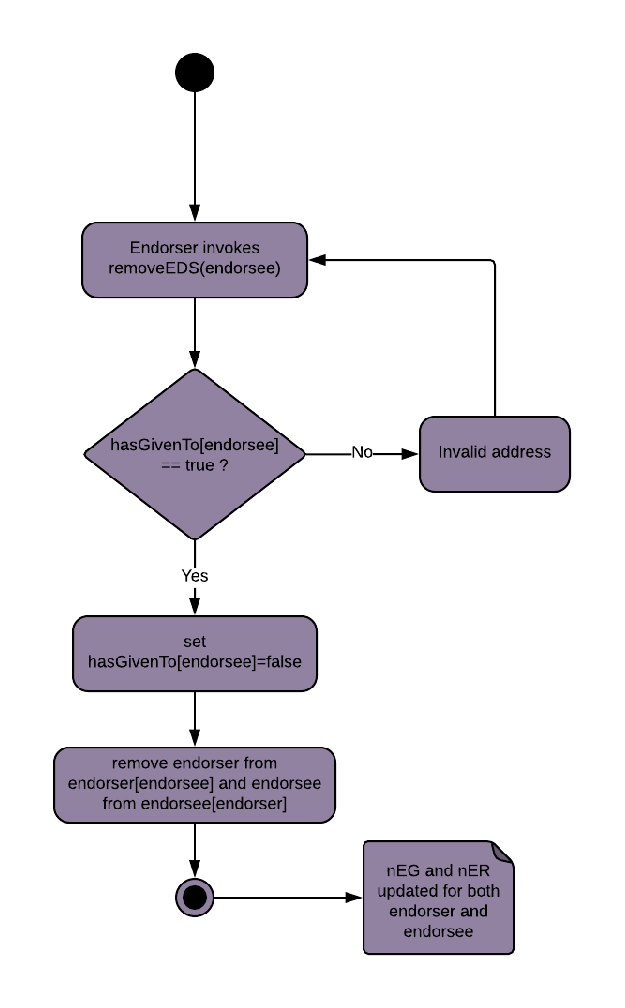
\includegraphics[width=0.5\textwidth]{Images/ActivityDiagramRemoveEDS.eps}
%	\caption{Activity diagram for removing endorsement}
%	\label{fig:removeEds}
%\end{figure}
%'Marketplace' contract was written to test the endorsement network on a
%transactional network. However, when deploying endorsement system in the real
%world, other transactional network/online systems are assumed to have their
%reputation platform. The reputation platform should have assigned a score to
%the corresponding users based on the behavior on that network. The endorsement
%system can act as additional conformity for deciding on a transaction. Say,
%Alice is registered on Endorsement network and has made a decent score. If she
%wants to sell a product on Marketplace(or any other transactional network), she
%can claim about her score and anyone who wants to buy from Alice can verify the
%claim by checking the score that corresponds to her public address. If both
%Alice and buyer are registered on the endorsement network on the blockchain,
%they can send a pre-transaction message to each other to verify that Alice is
%who she claims to be and vice-versa. In case the buyer is not registered on the
%endorsement network then Alice can prove the claim by signing a cryptographic
%challenge with her private key. 
%\begin{figure}
%	\centering
%	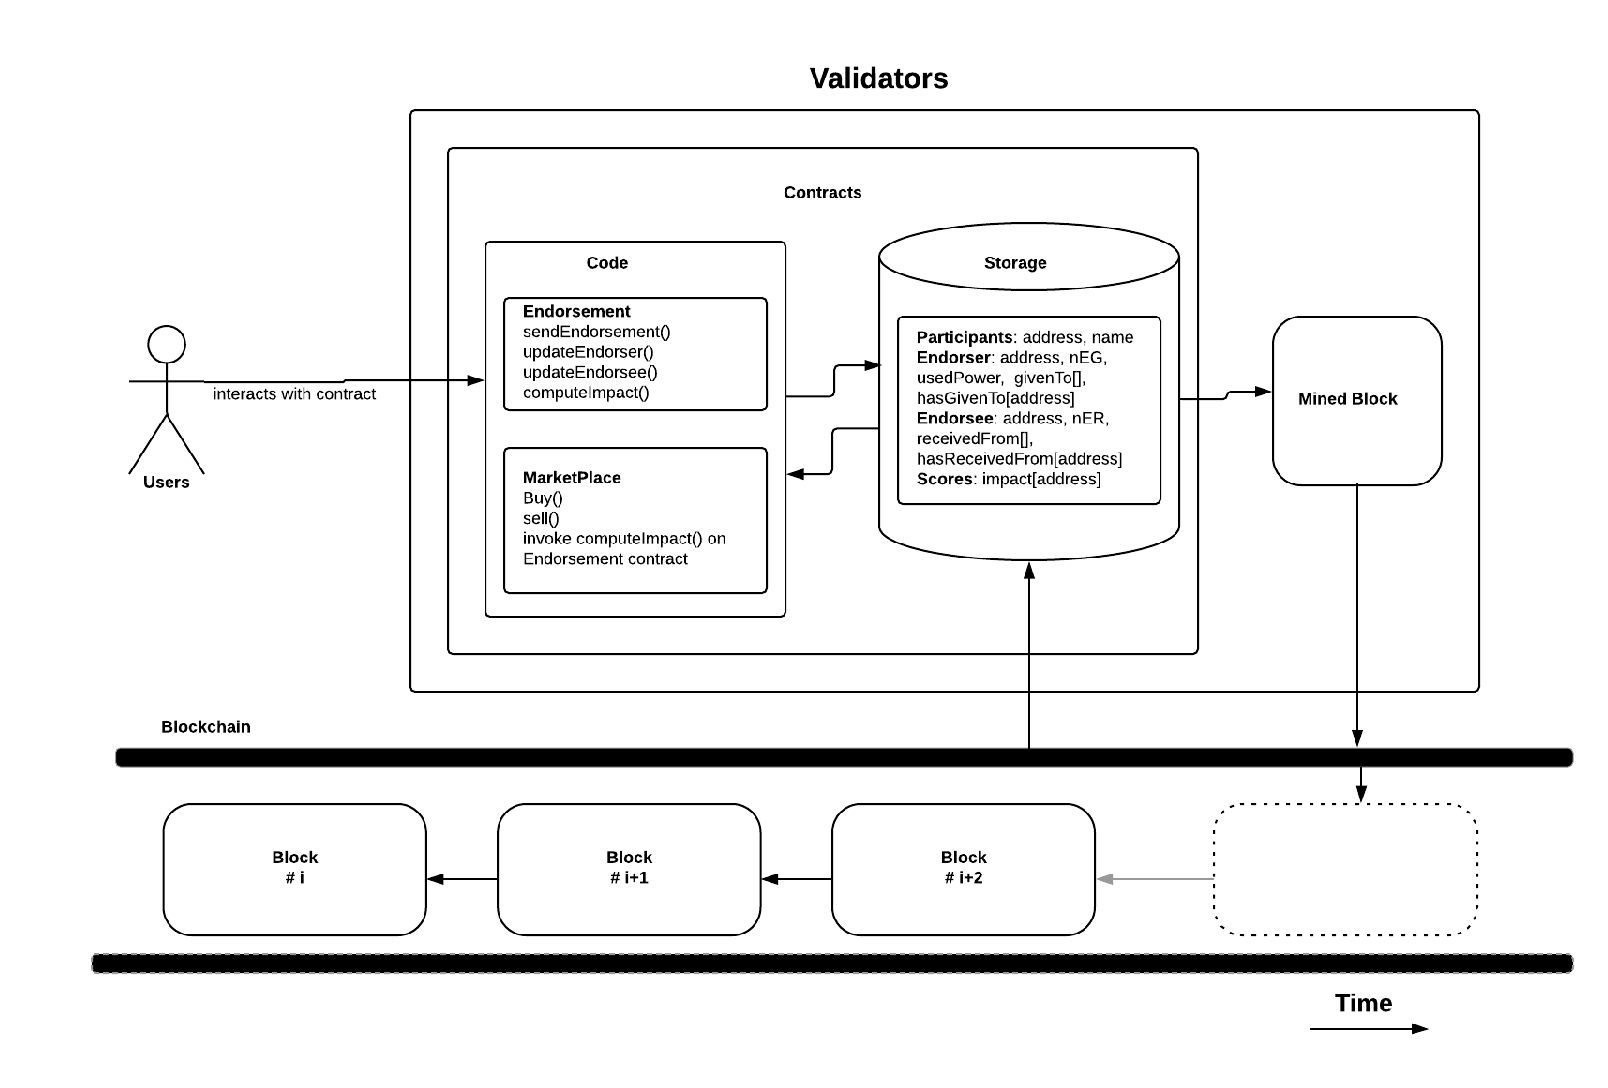
\includegraphics[width=1.0\textwidth]{Images/SmartContractsEDSMarketPlace.eps}
%	\caption{Smart contract system}
%	\label{fig:smartcontracts}
%\end{figure}

\subsection{Data and variables on and off blockchain}
For the endorsement system, the data required to identify the users are stored
on the blockchain. However, it preserves the anonymity requirement mentioned in
Section~\ref{ch:UserStories}, as the publicly available information only links
to the pseudonymous identity. The trust scores of an individual are just linked
with the public key hash (account identifier). When sending a request to join
the endorsement network, the user is asked to input a username. Unless a user
explicitly wants to give out their real name, they are not required to be
linked to real-world identity in any way. The current implementation of the
endorsement system allows a user to only have a username as their profile
information. Other variables related to trust scores are updated based on the
endorsement interaction they make with others on the network. It is possible
that storage requirements grow for reasons such as users willing to input more
information about them (e.g., other online accounts, address) or the need to
formulate complex trust metrics. As the data storage requirement increases, the
amount of gas required for the transaction also increases. As such, we could
use off-blockchain storage solution such as IPFS, Swarm~\cite{benet2014ipfs}.
The data can be stored off blockchain, and only the hash that points to the
specific file in IPFS can be stored on the blockchain. Also, client-side assets
(HTML, js) can be stored using the similar approach on the distributed
off-chain file system, storing only the hash of the file location on the
blockchain. 

\subsection{Blockchain and Consensus algorithms}\label{subsec:bcConsensus}
The proposed blockchain platform for the endorsement system is Ethereum, a
public, permissionless blockchain setup. As a public and permissionless
network, it allows any nodes to collect transactions and act as a writer. The
consensus mechanism that is generally used in a permissionless setting is
\ac{PoW}. As mentioned earlier, \ac{PoW} is computationally expensive and wasteful.
Using other consensus mechanisms such as delegated proof of stake requires
finding enough trustworthy validators that can act as a leader or a master node
which can be given authority to vote on behalf of the community.  The
endorsement system is meant to be a voluntary contribution network where anyone
is free to join and endorse whoever they wish to. The participants do not
necessarily know each other. Therefore, no "one" node can be trusted to collect
everyone's transaction and make a final commit.
Gochain~\footnote{https://gochain.io/} has mentioned the use of PoR
(Proof-Of-Reputation) as a consensus mechanism in its ethereum based blockchain
platform. The basic idea here is to allow participants on the network that have
a high reputation to sign the block. It builds on the theory that it is not
worthwhile for a reputed node to tarnish the current reputation that took some
time and effort to create. The endorsement system is designed to assign a
global reputation score to each entity and could use PoR. Since reputation
scores are significant to maintain, the nodes that have an impact score within
some given range could be trusted to validate and sign the blocks of
transactions. PoR on endorsement system can only be used if the endorsement
that results in an impact value becomes a valuable asset over time through
extensive use to be used on a transaction network. However, starting the
endorsement system with only PoR is not recommended as the behavior of
participants cannot be anticipated from the beginning. Only after several
endorsement interactions and analysis of the nodes on the network and updating
the trust score constantly based on transaction feedback, the trust score can
become more reliable. \par
Therefore, the recommended consensus algorithm for the endorsement system is
\ac{PoW} despite its limitations. Various alternatives to \ac{PoW} and
consensus related researches focusing on current problems (e.g.,  transaction
speed, transaction size, throughput) are under development.
Hashgraph~\cite{baird2016hashgraph} proposes the recent advancement in
consensus engine that claims to be fair (in the order of transactions), fast
(transaction processing) and Byzantine fault tolerant. It is based on gossip
protocol, where nodes gossip about transactions and gossips with each other,
and the gossip eventually leads to all the nodes in the network having the same
information. It offers mathematical proof of the total order of transactions
with less communication overhead. However, the hashgraph conundrum is that
their software is patented unlike other developments in the similar space. A
developer must pay for making an API call using micropayment of the platform.
Endorsement system can also be used on a permissioned setting, much like sovrin
does~\cite{tobin2016inevitable}. Sovrin introduces a steward node who is
trusted based on a signed agreement with
sovrin~\footnote{https://sovrin.org/library/steward-agreement/} and has
received approval as trusted institutions. The concept of steward nodes might
be questionable regarding decentralization aspect of the network, but there are
cases when this level of decentralization is enough for the security of an
application. For instance, there can be a consortium of e-commerce platforms
that could agree on a specific set of protocols.  Validation of transactions
could be based on a voting mechanism that requires the consent of 2/3 of
trusted members. Doing so can significantly increase the transaction validation
time compared to \ac{PoW}.
%\begin{figure}[h]
%	\centering
%	\includegraphics[width=0.5\textwidth]{Images/ActivityDiagram.eps}
%	\caption{Activity Diagram for sending an endorsement}
%	\label{fig:activity}
%\end{figure}

%\subsection{Graph based algorithm for anomaly detection} %\section{Honest vs. Malicious Nodes} User profile : consistent
% declining reputation
% progressing reputation

% The idea is not to exclude malicious behavior in the network, rather include them 
% but give them no value. The endorsement power diminishes every time an entity 
% gives it to someone so the right thing to do for any entity would be to use 
% them wisely. 
% It can be analogous to a gameplay where a player is not restricted to 
% drink a life potion when his lifebar is full but he will waste it if he does with 
% no impact and when the time comes to use it, there won't be any more potion left. 
% drinking potion when you have full life 

%consensus algorithm - 
%what stops someone from making 250 nodes and just endorsing 
%themself.  - net flow rate convergence ,
% would detect this. as we can all 250 nodes are created just to endorse this one 
% node, and so those nodes value would soon converge to zero. 
 
 
%  Problem: What happens if someone plays well in the network for a long time and in 
%  the end decides to betray the whole network. (spy)


% The goal is : once a dishonest node is detected by reputation algorithm in a 
% transaction network, all their endorsement given or received is automatically removed 
% from the network so that will change the values in the dishonest node and other nodes 
% that were connected to it in the past. 

% net flow rate convergence can also be used to determine anomaly in the network. 

% incentivize honest behaviour.


%Model as interaction graph
%quantify endorsement as reputation score and translate to trust value
%mention reputation algorithm as necessary to be used on the n/w. 

%\section{Trust Metrics}

%central nodes, 
%How is trust measured?
%What is required for it to be a correct solution? 
%objective way of accepting or rejecting the work
%Every node keeps track of its neighbouring node and whenever an intera



%\section{Experimental Setup} \label{sec:sectionlabel}

%Test Network describe, no. of nodes, level of difficulty etc.

%\section{second section}
% It may include: Description of the methodological, theoretical, conceptual or empirical framework; design of the
% experiment; relevant steps of reasoning; data description and sources.

% Describe the approach and method(s) used to address the scientific problem. Also reflect on the particular choice of method and justify it.
